\section{Aturan Route di Flask}	
Kerangka kerja web modern menggunakan teknik route untuk membantu pengguna mengingat URL aplikasi. Berguna untuk mengakses halaman yang diinginkan secara langsung tanpa harus bernavigasi dari halaman beranda. Penggunaan route () dalam Flask digunakan untuk mengikat URL ke suatu fungsi. Routing merupakan suatu modul dalam sebuah aplikasi yang berfungsi untuk mengatur jalannya aplikasi yang berbasis web.

Dekorator python adalah fungsi yang digunakan untuk mengubah fungsi lainnya. Ketika fungsi yang didekorasi pada app.route dipanggil, dekorator dipanggil sebagai gantinya. Dekorator kemudian dapat mengambil tindakan, memodifikasi argumen, menghentikan eksekusi atau memanggil fungsi asli. Untuk membuat routing pada python flask langkah pertama pastikan teman-teman telah menginstall python dan telah menginstall package flask yang akan anda gunakan. Untuk struktur penulisan routing pada flask yaitu seperti pada listing \ref{lst:app}.
\lstinputlisting[caption=File app.py, label={lst:app}]{src/9/app.py}

Pada baris pertama flask adalah framework di sini, sedangkan Flask adalah tipe data kelas Python. Dengan kata lain, Flask adalah prototipe yang digunakan untuk membuat aplikasi web. setelah mengimpor Flask, maka perlu membuat turunan dari kelas Flask untuk aplikasi web yang akan di buat. Itulah yang dilakukan  app = Flask(\_\_name\_\_)  adalah variabel khusus yang mendapatkan nilai string "\_\_main\_\_" ketika Anda menjalankan skrip kode diatas.

@app.route adalah dekorator pada flask yang digunakan untuk mencocokkan URL dan  memberi tahu Flask URL apa yang harus digunakan untuk melihat fungsi di aplikasi Flask. Kemudian mendefinisikan fungsi yang mengembalikan string "Hello World!". Fungsi itu dipetakan ke URL beranda ‘/’. Fungsi hello() digunakan untuk menghasilkan URL dan kemudian Return “Hello world” mengembalikan pesan yang ingin di tampilkan di browser pesan yang kan di tampilkan pada browser adalah ‘Hello World’.

Karena \_\_name\_\_ akan sama dengan "\_\_main\_\_" dan metode app.run () akan dieksekusi. Teknik ini memungkinkan programmer untuk mengontrol perilaku skrip. Perhatikan juga bahwa ada parameter debug ke true. Itu akan mencetak kemungkinan kesalahan Python di halaman web membantu untuk melacak kesalahan. Namun, dalam lingkungan produksi, jika ingin mengaturnya ke False untuk menghindari masalah keamanan.
\begin{enumerate}
\item Simpan script diatas dengan nama app.py kemudian jalankan menggunakan command prompt seperti pada gambar \ref{fig:phw}.
\begin{figure}[!htbp]
	\centerline{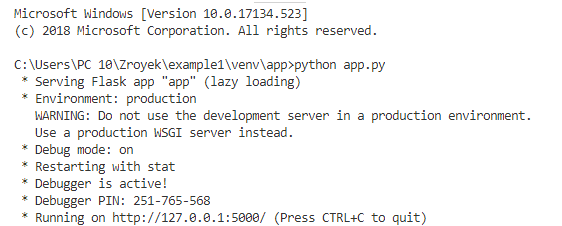
\includegraphics[width=0.85\textwidth]{figures/9/phw.PNG}}
	\caption{Pengujian helloworld}
	\label{fig:phw}
\end{figure}

\item Setelah itu akan muncul pemberitahuan bahwa Flask telah berjalan di localhost.
\item Jalankan program di http://127.0.0.1:5000/ maka akan muncul tampilan seperti pada gambar \ref{fig:hphw}.
\begin{figure}[!htbp]
	\centerline{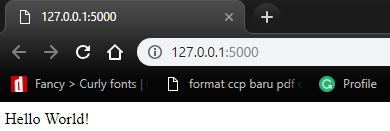
\includegraphics[width=0.85\textwidth]{figures/9/hphw.PNG}}
	\caption{Hasil Pengujian helloworld}
	\label{fig:hphw}
\end{figure}

\item @app.route harus selalu menjadi dekorator tampilan terluar. Didalam dekorator @app.route("/"), slash (‘/’) artinya di mainroot anda bisa menambahkan filled apa saja yang ingin anda tambahkan misalnya @app.route("/contoh"). 
\end{enumerate}

\section{Aturan URL di Flask}
Selain itu anda juga bisa memodifikasinya sesuai keinginan anda agar lebih mudah untuk mengingat suatu URL aplikasi seperti pada listing \ref{lst:appt}.
\lstinputlisting[caption=Contoh File app.py, label={lst:appt}]{src/9/appt.py}
\begin{enumerate}
\item @app.route("/contoh") digunakan sebagai Url yang nanti akan anda panggil di browser.
\item Simpan script code diatas kemudian running kembali kode tersebut seperti pada gambar \ref{fig:ujiurl}.
\begin{figure}[!htbp]
	\centerline{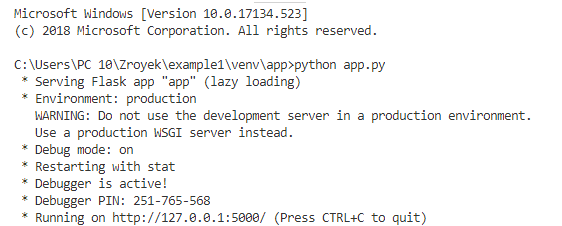
\includegraphics[width=0.85\textwidth]{figures/9/ujiurl.PNG}}
	\caption{Pengujian url contoh}
	\label{fig:ujiurl}
\end{figure}

\item Setelah itu akan muncul pemberitahuan bahwa Flask telah berjalan di localhost.
\item Jalankan program di http://127.0.0.1:5000/  maka akan muncul tampilan seperti pada gambar \ref{fig:hujiurl}.
\begin{figure}[!htbp]
	\centerline{
\includegraphics[width=0.85\textwidth]{figures/9/hujiurl.PNG}}
	\caption{Hasil Pengujian url contoh}
	\label{fig:hujiurl}
\end{figure}

\item Error terjadi dikarnakan URL pada direktori @app.route ditambahkan dengan ("/contoh") sehingga URL yang diminta tidak ditemukan di server. 
\item Maka dari itu tambahkan /contoh pada Url flask, seperti ini  http://127.0.0.1:5000/contoh kemudian refresh web browser, maka akan muncul tampilan web seperti pada gambar \ref{fig:hujiurlc}.
\begin{figure}[!htbp]
	\centerline{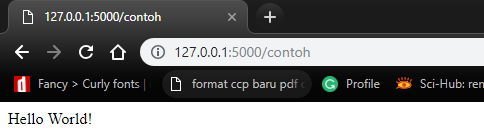
\includegraphics[width=0.85\textwidth]{figures/9/hujiurlc.PNG}}
	\caption{Hasil Pengujian url contoh}
	\label{fig:hujiurlc}
\end{figure}
\end{enumerate}

\section{Berbagai Macam Jenis Kreasi URL di Flask}
Anda bisa kreasikan URL pada flask untuk membantu pengguna mengingat URL aplikasi. Selain URL /contoh seperti gambar diatas anda bisa memanage Url dalam flask, misalnya anda akan mencoba parameter get pada URL flask seperti pada listing \ref{lst:appvar}.
\lstinputlisting[caption=Contoh File app.py variabel, label={lst:appt}]{src/9/appvar.py}
\begin{enumerate}
\item URL yang ada  pada direktori @app.route di ubah menjadi sebuah variable (‘/<contoh>’), artinya apapun yang ditulis setalah slash (/) pada browser maka akan di keluarkan di browser. 
\item Return contoh2 akan mengembalikan fungsi yang sudah dibuat dna akan menampilkannya ke browser.
\item Simpan script code diatas kemudian running kembali kode tersebut seperti pada gambar \ref{fig:ujivar}.
\begin{figure}[!htbp]
	\centerline{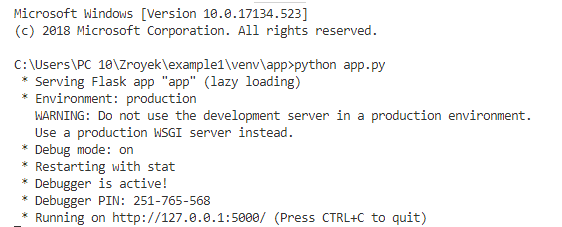
\includegraphics[width=0.85\textwidth]{figures/9/ujivar.PNG}}
	\caption{Pengujian variabel}
	\label{fig:ujivar}
\end{figure}

\item Setelah itu akan muncul pemberitahuan bahwa Flask telah berjalan di localhost.
\item Jalankan program di http://127.0.0.1:5000/ kemudian tuliskan kata atau kalimat yang di inginkan setealah slash (/) seperti pada gambar \ref{fig:hujivar1} dan \ref{fig:hujivar2}.
\begin{figure}[!htbp]
	\centerline{
\includegraphics[width=0.85\textwidth]{figures/9/hujivar1.PNG}}
	\caption{Hasil Pengujian Variabel 1}
	\label{fig:hujivar1}
\end{figure}

\begin{figure}[!htbp]
	\centerline{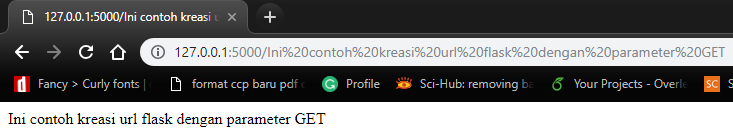
\includegraphics[width=0.85\textwidth]{figures/9/hujivar2.PNG}}
	\caption{Hasil Pengujian Variabel 2}
	\label{fig:hujivar2}
\end{figure}

\item Apa yang terjadi jikalau anda menuliskan yang aneh pada url di web browser misalnya seperti pada gambar \ref{fig:hujivar3}, \ref{fig:hujivar4}, \ref{fig:hujivar5}, \ref{fig:hujivar6}, dan \ref{fig:hujivar7}.
\begin{figure}[!htbp]
	\centerline{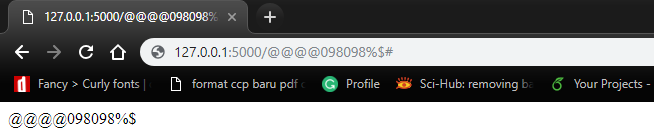
\includegraphics[width=0.85\textwidth]{figures/9/hujivar3.PNG}}
	\caption{Hasil Pengujian Variabel 3}
	\label{fig:hujivar3}
\end{figure}

\begin{figure}[!htbp]
	\centerline{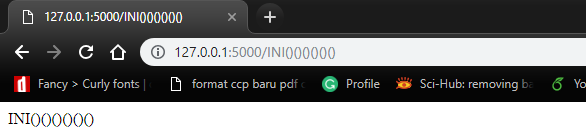
\includegraphics[width=0.85\textwidth]{figures/9/hujivar4.PNG}}
	\caption{Hasil Pengujian Variabel 4}
	\label{fig:hujivar4}
\end{figure}

\begin{figure}[!htbp]
	\centerline{
\includegraphics[width=0.85\textwidth]{figures/9/hujivar5.PNG}}
	\caption{Hasil Pengujian Variabel 5}
	\label{fig:hujivar5}
\end{figure}

\begin{figure}[!htbp]
	\centerline{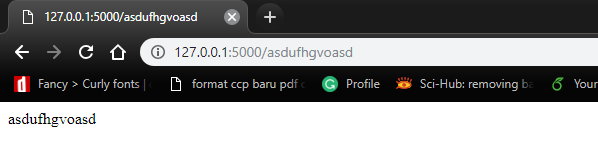
\includegraphics[width=0.85\textwidth]{figures/9/hujivar6.PNG}}
	\caption{Hasil Pengujian Variabel 6}
	\label{fig:hujivar6}
\end{figure}

\begin{figure}[!htbp]
	\centerline{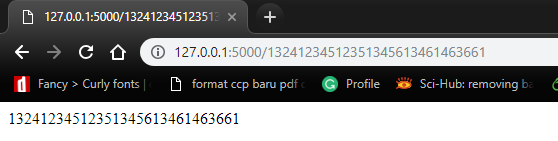
\includegraphics[width=0.85\textwidth]{figures/9/hujivar7.PNG}}
	\caption{Hasil Pengujian Variabel 7}
	\label{fig:hujivar7}
\end{figure}

\item Itulah tadi contoh sederhana pada URL flask dengan menggunakan Parameter Get.
\item Selain contoh diatas anda akan coba menggunakan simbol-simbol untuk mengganti alamat url yang akan anda panggil di browser 
\item Misalnya seperti pada listing \ref{lst:appsim}.
\lstinputlisting[caption=Contoh File app.py simbol, label={lst:appsim}]{src/9/appsim.py}

\item Simpan script code diatas kemudian running kembali kode tersebut seperti pada gambar \ref{fig:ujisim}.
\begin{figure}[!htbp]
	\centerline{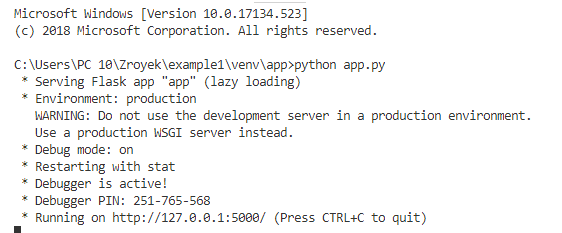
\includegraphics[width=0.85\textwidth]{figures/9/ujisim.PNG}}
	\caption{Pengujian simbol}
	\label{fig:ujisim}
\end{figure}

\item Setelah itu akan muncul pemberitahuan bahwa Flask telah berjalan di localhost.
\item Jalankan program di http://127.0.0.1:5000/  maka akan muncul halaman web seperti pada gambar \ref{fig:hujisim1}.
\begin{figure}[!htbp]
	\centerline{
\includegraphics[width=0.85\textwidth]{figures/9/hujisim1.PNG}}
	\caption{Hasil Pengujian simbol 1}
	\label{fig:hujisim1}
\end{figure}

\item Maka akan terjadi eror seperti ini, ini terjadi dikarnakan URl yang di panggil tidak di temukan oleh server. 
\item Dalam scrip kode yang sudah anda buat anda membuat url baru dengan kata (coba\%symbol), sekarang anda coba menambahkan kata tersebut setelah slash di alamat url web  http://127.0.0.1:5000/coba\%symbol  seperti pada gambar \ref{fig:hujisim2}.
\begin{figure}[!htbp]
	\centerline{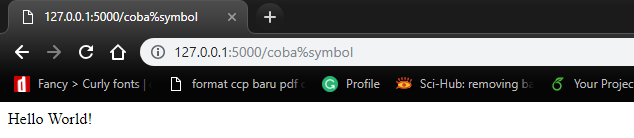
\includegraphics[width=0.85\textwidth]{figures/9/hujisim2.PNG}}
	\caption{Hasil Pengujian simbol 2}
	\label{fig:hujisim2}
\end{figure}

\item Anda bisa mencoba dengan menambahkan beberapa code html kedalam scrip code yang sudah anda buat, misalnya tulisan yang akan di tampilkan tampak lebih besar, contoh seperti pada listing \ref{lst:appht}.
\lstinputlisting[caption=Contoh File app.py heading text, label={lst:appht}]{src/9/appht.py}

\item return "<h1>Hello World!<h1>"  ini akan menampilkan tulisan Hello World dengan ukuran yang lebih besar, simpan code diatas kemudian jalankan.
\item Simpan skrip kode diatas kemudian jalankan kembali program seperti pada gambar \ref{fig:ujiht}.
\begin{figure}[!htbp]
	\centerline{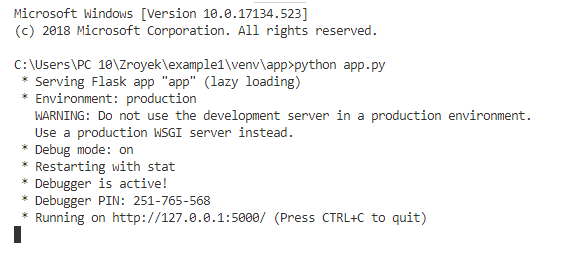
\includegraphics[width=0.85\textwidth]{figures/9/ujiht.PNG}}
	\caption{Pengujian heading text}
	\label{fig:ujiht}
\end{figure}

\item Setelah itu akan muncul pemberitahuan bahwa Flask telah berjalan di localhost.
\item Jalankan program di http://127.0.0.1:5000/  maka akan muncul halaman web seperti pada gambar \ref{fig:hujiht}.
\begin{figure}[!htbp]
	\centerline{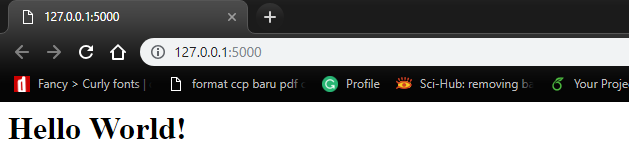
\includegraphics[width=0.85\textwidth]{figures/9/hujiht.PNG}}
	\caption{Hasil Pengujian heading text}
	\label{fig:hujiht}
\end{figure}

\item Anda juga bisa kreasikan @app.route dan url yang berbeda beda dalam 1 file.py misalnya seperti pada listing \ref{lst:appcl}.
\lstinputlisting[caption=Contoh File app.py contoh lain, label={lst:appcl}]{src/9/appcl.py}

\item Simpan skrip kode diatas kemudian jalankan kembali program seperti pada gambar \ref{fig:ujicl}.
\begin{figure}[!htbp]
	\centerline{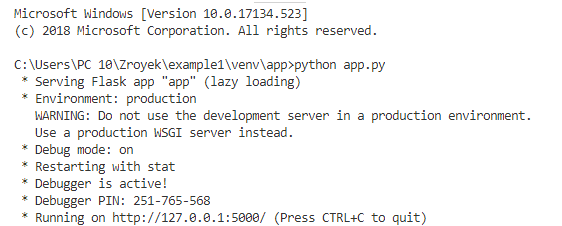
\includegraphics[width=0.85\textwidth]{figures/9/ujicl.PNG}}
	\caption{Pengujian contoh lain}
	\label{fig:ujicl}
\end{figure}

\item Setelah itu akan muncul pemberitahuan bahwa Flask telah berjalan di localhost.
\item Jalankan program di http://127.0.0.1:5000/ maka akan muncul halaman web seperti pada gambar \ref{fig:hujicl1}.
\begin{figure}[!htbp]
	\centerline{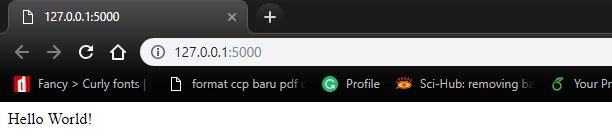
\includegraphics[width=0.85\textwidth]{figures/9/hujicl1.PNG}}
	\caption{Hasil Pengujian contoh lain 1}
	\label{fig:hujicl1}
\end{figure}

\item Jika anda tambahkan /anu seperti didalam scrip kode pada alamat url http://127.0.0.1:5000/anu maka tampilannya akan seperti pada gambar \ref{fig:hujicl2}.
\begin{figure}[!htbp]
	\centerline{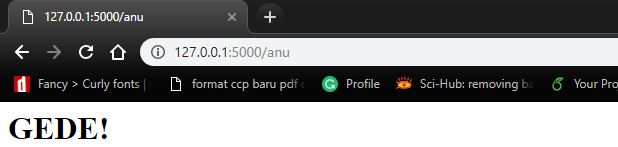
\includegraphics[width=0.85\textwidth]{figures/9/hujicl2.PNG}}
	\caption{Hasil Pengujian contoh lain 2}
	\label{fig:hujicl2}
\end{figure}

\item Dan yang yetakhir menggunakan symbol \% pada URL yang sudah di buat pada skrip kode maka tampilan pada web browser akan seperti pada gambar \ref{fig:hujicl3}.
\begin{figure}[!htbp]
	\centerline{
\includegraphics[width=0.85\textwidth]{figures/9/hujicl3.PNG}}
	\caption{Hasil Pengujian contoh lain 3}
	\label{fig:hujicl3}
\end{figure}

\item Di flask anda bisa sesuka hati mengatur URL apa yang akan di gunakan untuk memanggil sebuah progam yang akan dijalankan, dengan tujuan untuk lebih mempermudah si user dalam mengingat url aplikasi seperti pada listing \ref{lst:appcc}.
\lstinputlisting[caption=Contoh File app.py cobacoba 1, label={lst:appcc}]{src/9/appcc.py}
\item Simpan skrip kode diatas kemudian jalankan kembali program seperti pada gambar \ref{fig:ujicc1}.
\begin{figure}[!htbp]
	\centerline{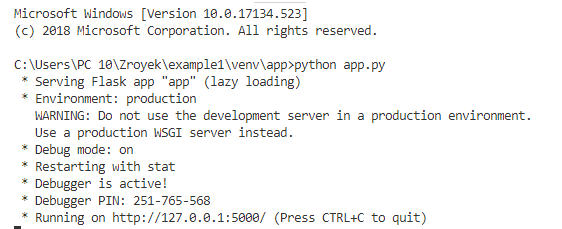
\includegraphics[width=0.85\textwidth]{figures/9/ujicc1.PNG}}
	\caption{Pengujian cobacoba 1}
	\label{fig:ujicc1}
\end{figure}

\item Setelah itu akan muncul pemberitahuan bahwa Flask telah berjalan di localhost.
\item Jalankan program di http://127.0.0.1:5000/cobalagi maka akan muncul halaman web seperti pada gambar \ref{fig:hujicc1}.
\begin{figure}[!htbp]
	\centerline{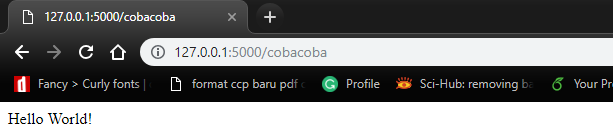
\includegraphics[width=0.85\textwidth]{figures/9/hujicc1.PNG}}
	\caption{Hasil Pengujian cobacoba 1}
	\label{fig:hujicc1}
\end{figure}

\item Pada listing \ref{lst:appcc2}.
\lstinputlisting[caption=Contoh File app.py cobacoba 2, label={lst:appcc2}]{src/9/appcc2.py}

\item Simpan skrip kode diatas kemudian jalankan kembali program seperti pada gambar \ref{fig:ujicc2}.
\begin{figure}[!htbp]
	\centerline{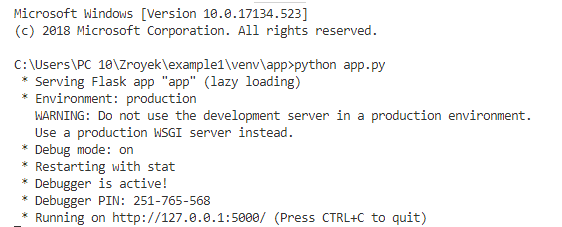
\includegraphics[width=0.85\textwidth]{figures/9/ujicc2.PNG}}
	\caption{Pengujian cobacoba 2}
	\label{fig:ujicc2}
\end{figure}

\item Setelah itu akan muncul pemberitahuan bahwa Flask telah berjalan di localhost.
\item Jalankan program di http://127.0.0.1:5000/cobalagi maka akan muncul halaman web seperti pada gambar \ref{fig:hujicc2}.
\begin{figure}[!htbp]
	\centerline{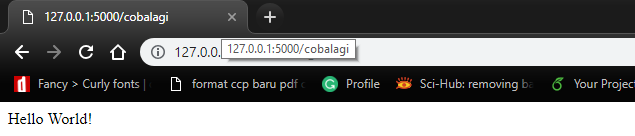
\includegraphics[width=0.85\textwidth]{figures/9/hujicc2.PNG}}
	\caption{Hasil Pengujian cobacoba 2}
	\label{fig:hujicc2}
\end{figure}

\item Contoh yang selanjutnya adalah seperti pada listing \ref{lst:appsl}.
\lstinputlisting[caption=Contoh File app.py sekali lagi, label={lst:appsl}]{src/9/appsl.py}

\item Simpan skrip kode diatas kemudian jalankan kembali program seperti pada gambar \ref{fig:ujisl}.
\begin{figure}[!htbp]
	\centerline{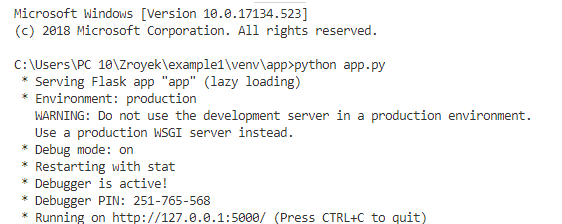
\includegraphics[width=0.85\textwidth]{figures/9/ujisl.PNG}}
	\caption{Pengujian sekali lagi}
	\label{fig:ujisl}
\end{figure}

\item Setelah itu akan muncul pemberitahuan bahwa Flask telah berjalan di localhost.
\item Jalankan program di http://127.0.0.1:5000/cobalagi maka akan muncul halaman web seperti pada gambar \ref{fig:hujisl}.
\begin{figure}[!htbp]
	\centerline{
\includegraphics[width=0.85\textwidth]{figures/9/hujisl.PNG}}
	\caption{Hasil Pengujian sekali lagi}
	\label{fig:hujisl}
\end{figure}

\item Pada listing \ref{lst:appcc3}.
\lstinputlisting[caption=Contoh File app.py cobacoba 3, label={lst:appcc3}]{src/9/appcc3.py}

\item Selama URL ada di dalam decorator flask (@app.route) apapun URL yang dibuat dan kemudian di panggil ke browser maka akan menampilkan output sesuai dengan apa yang anda ingin tampilkan dengan mngembalikan fungsi yang sudah dibuat. Jika URL yang dimasukan kedalam alamt web tidak sesuai maka akan terjadi eror yang mana URL yang di minta tidak ditemukan oleh server flask. Kecuali URL yang di buat menggunakan variable seperti contoh sebelumnya, flask akan menampilkan string yang ditulis pada alamat url di browser.

\item Pada contoh sebelumnya parameter variable yang sudah dibuat menjadi parameter get pada flask python. flask memberikan kemudahan bagi para user untuk mengakses alamat web dengan menggunakan URL yang bisa di ubah ubah sesuka hati menggunakan karakter-karakter aneh didalam url itu salah satu kelebihan flask yang merupakan framework pada python yang sangat customizable bagi si pengguna flask python.  Itulah tadi contoh sederhana dan penjelasn Route dan URL di Flask.

\end{enumerate}

\section{Penanganan Error}
\subsection{Error 1}
Pada listing \ref{lst:flc}.
\lstinputlisting[caption=File flasklivechart.py , label={lst:flc}]{src/9/flasklivechart.py}

\begin{enumerate}
\item Simpan skrip kode diatas kemudian namakan file tersebut menjadi flasklivechart.py, jalankan file tersebut menggunakan cmd dengan menuliskan perintah python flasklivechart.py seperti pada gambar \ref{fig:ujiflc}.
\begin{figure}[!htbp]
	\centerline{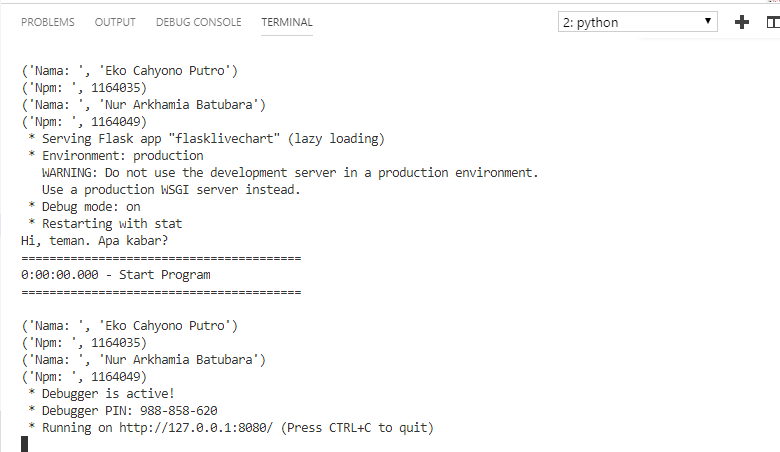
\includegraphics[width=0.85\textwidth]{figures/9/ujiflc.PNG}}
	\caption{Pengujian file flasklivechart.py}
	\label{fig:ujiflc}
\end{figure}

\item Setelah itu akan muncul pemberitahuan bahwa Flask telah berjalan di localhost.
\item Jalankan program di http://127.0.0.1:8080 kemudian akan muncul tampilan seperti berikut:
\item Akan tetapi terdapat suatu masalah pada halaman home seperti pada gambar \ref{fig:hujiflc}.
\begin{figure}[!htbp]
	\centerline{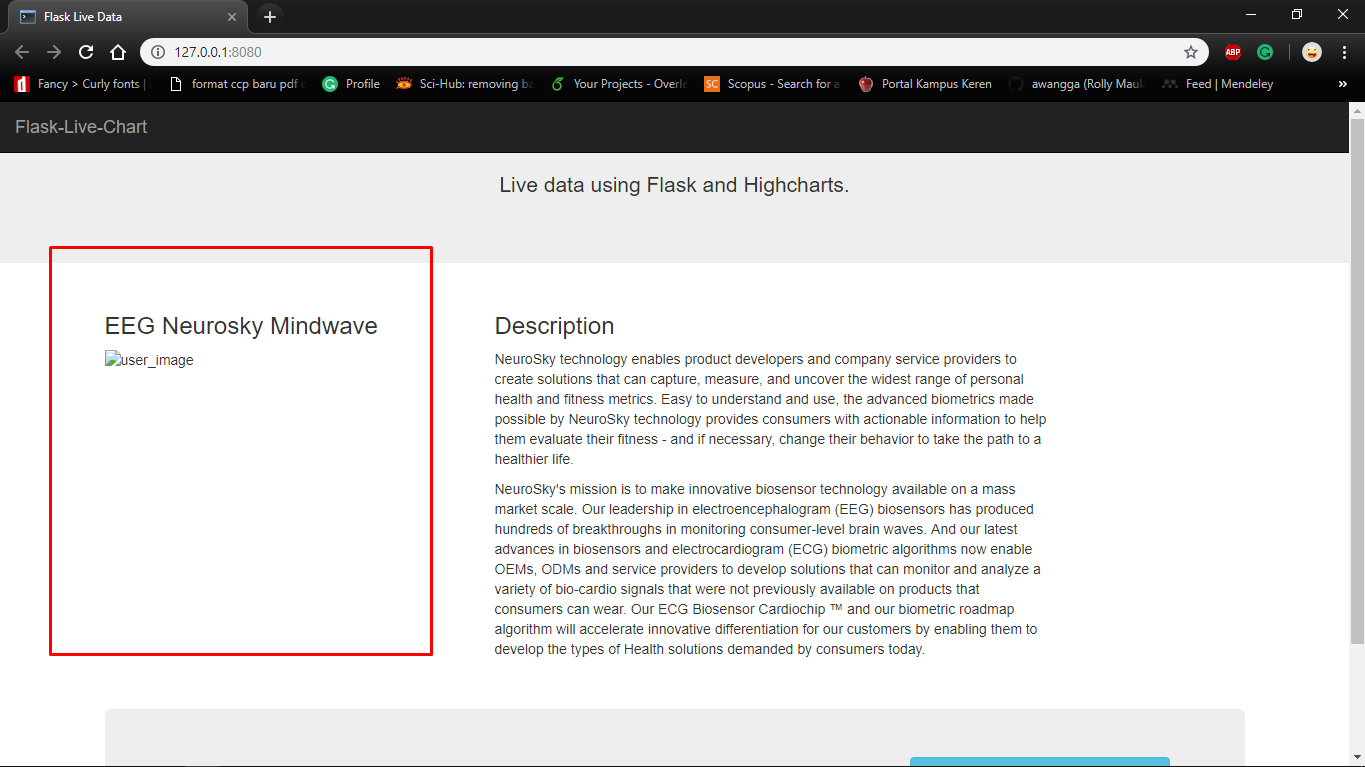
\includegraphics[width=0.85\textwidth]{figures/9/hujiflc.PNG}}
	\caption{Hasil Pengujian file flasklivechart.py}
	\label{fig:hujiflc}
\end{figure}

\item Muncul eror seperti ini pada Command Prompt seperti pada gambar \ref{fig:errflc}.
\begin{figure}[!htbp]
	\centerline{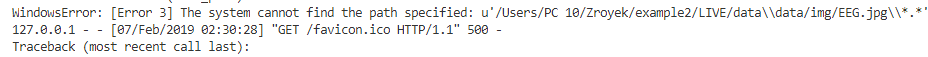
\includegraphics[width=0.85\textwidth]{figures/9/errflc.PNG}}
	\caption{CMD file flasklivechart.py}
	\label{fig:errflc}
\end{figure}

\item Dan pada command Prompt ditemukan eror seperti berikut:
\item Windows Eror: [Error 3] The system cannot find the path specified: u'/Users/PC 10/Zroyek/example2/LIVE/data\\data/img/EEG.jpg\\*.*'
\end{enumerate}

\subsection{Error 2}
\begin{enumerate}
\item Melanjutkan pembahasan Error 1 yang saling berkaitan dengan Error 2 ini
\item Masalah yang terjadi pada aplikasi yang sudah dibuat adalah gambar di program flask tidak muncul,  function yang ada dalam kode program adalah seperti pada listing \ref{lst:flcedit}.
\lstinputlisting[caption=File flasklivechart.py edit , label={lst:flcedit}]{src/9/flcedit.py}

\item fungsi def img() dan def show\_index() saling berhubungan karena fungi show\_index() akan menampilkan gambar dengan merender file index.html yang ada pada folder templates dan funsi img() akan menggabungkan folder dan menentukan path yang digunakan serta akan menempilkan gambar di web browser.
\item Disini kita akan mencoba memodifaki kode yang digukan untuk menampilkan gambar pada halaman HOME agar gambar dapat di tampilkan di browser.
\item Dan untuk struktur projek yang di kerjakan adalah seperti pada gambar \ref{fig:strpro}.
\begin{figure}[!htbp]
	\centerline{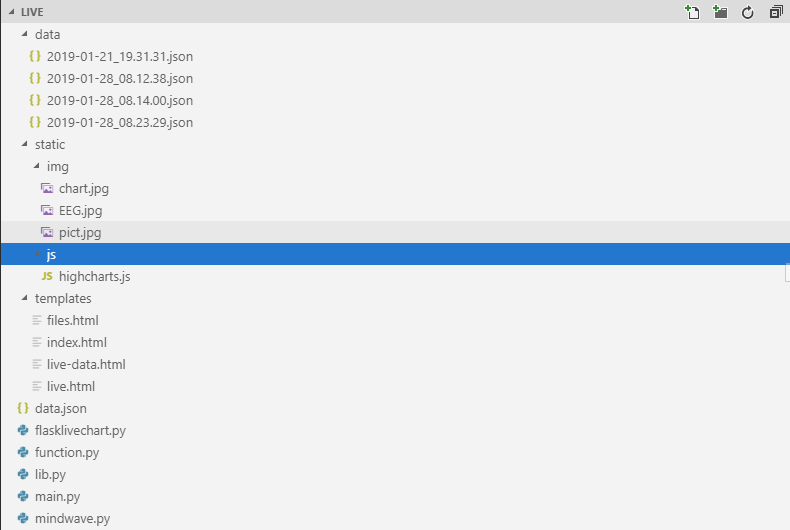
\includegraphics[width=0.85\textwidth]{figures/9/strpro.PNG}}
	\caption{Struktur Projek}
	\label{fig:strpro}
\end{figure}

\item Dalam hasil yang ditampilkan windows error mengatakan  bahwa  sistem tidak mampu menemukan jalur yang ditentukan.
\item Maksut jalur disini adalah path yang dugunakan utnuk mendeteksi dimana file gambar yang akan di tampilkan berada.
\item Dalam projek flask yang sudah di buat file img terdapat pada folder img yang disimpan didalam folder static dan gambar yang akan di tampilkan di web browser adalah gambar yang bernama EEG.jpg seperti pada gambar \ref{fig:alat}.
\begin{figure}[!htbp]
	\centerline{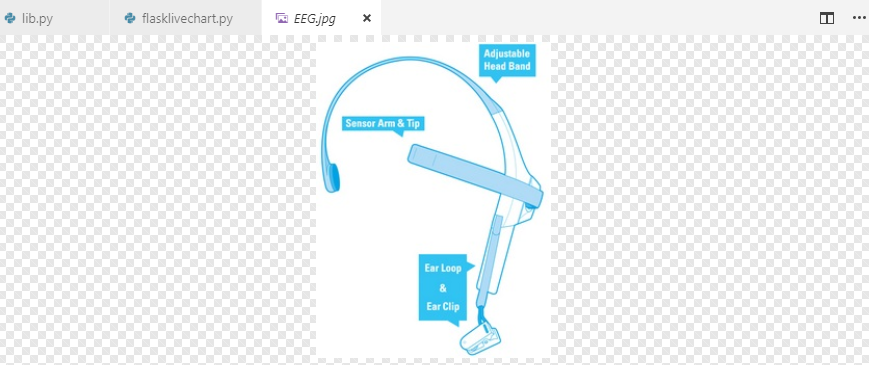
\includegraphics[width=0.85\textwidth]{figures/9/alat.PNG}}
	\caption{Alat yang akan ditampilkan}
	\label{fig:alat}
\end{figure}

\item Function yang menentukan path gambar adalah seperti pada listing \ref{lst:flcel}.
\lstinputlisting[caption=File flasklivechart.py edit , label={lst:flcel}]{src/9/flcel.py}

\item Setelah diteliti ada yang salah pada os.path.join, bukannya menggabungkan folder yang menyimpan gambar malah menggabungkan folder yang lain. 
\item Didalam folder ‘data’ tidak ada folder img yang menyimpan gambar EEG.jpg melainkan folder satic yang didalamnya terdapar folder img yang menyimpan gambar EEG.jpg 
\item Jadi yang harus kita lakukan adalah mengganti ‘data’ dengan ‘static’ karena folder img tada didalam folder static yang  menyimpan gambar EEG.jpg 
\item PEOPLE\_FOLDER = os.path.join('static', 'img')
\end{enumerate}